\documentclass[10pt]{article}
\usepackage{../../local}


\newcommand{\classcode}{Physics 112}
\newcommand{\classname}{Thermal Physics and Statistical Mechanics}
\renewcommand{\maketitle}{%
\hrule height4pt
\large{Eric Du \hfill \classcode}
\newline
\large{HW 07} \Large{\hfill \classname \hfill} \large{\today}
\hrule height4pt \vskip .7em
\normalsize
}
\linespread{1.1}
\begin{document}
	\maketitle
	\section*{Problem 1}
	Consider a parallel plate capacitor of capacitance $C$. From E\&M we know that when the capacitor has 
	charge $Q$, it has electrostatic energy \( E(Q) = \frac{Q^2}{2C}\). If the two plates are connected
	via a resistive wire at temperature \(T\), \(Q\) will fluctuate due to thermal motion of electrons. We 
	can think of the charge \(Q\) as a degree of freedom in equilibrium with a bath at temperature \(T\), 
	governed by the Boltzmann distribution 
	\[
		P(Q) = \frac{1}{Z} e^{-\beta \frac{Q^2}{2C}}
	\] 
	\begin{enumerate}[label=\alph*)]
		\item Assuming the charge \(Q \) is a continuous variable, use your knowledge of Gaussian integrals to 
			obtain \(Z\) and the thermal averages \(\mean{Q}, \mean{E}, \mean{Q^2}\) as functions of \(T\).

			\begin{solution}
				Here we first compute \(Z\) by setting the integral to equal 1:
				\[
					1 = \iinf P(Q) dQ = \iinf \frac{1}{Z}e^{-\beta Q / 2C} dQ  \implies 
					Z = \iinf e^{-\beta Q^2/2C} dQ
				\] 
				Now let \(x = \sqrt{\frac{\beta}{2C}} Q\), so we have: 
				\begin{align*}
					Z &= \iinf e^{-x^2} \cdot \sqrt{\frac{2C}{\beta}} dx \\
					&= \sqrt{\frac{2C}{\beta}} \sqrt{\pi}  \\
					&= \sqrt{\frac{2\pi C}{\beta}} 
				\end{align*}
				With this, we can begin by calculating \(\mean{Q}\) :
				\[
					\mean{Q} = \iinf Q P(Q) = \iinf \frac{Q}{Z}e^{-\beta Q^2/2C} dQ = 
					\sqrt{\frac{\beta}{2 \pi C}} 
					\underbrace{\iinf Qe^{-\beta Q^2 / 2C} dQ}_{\text{odd integrand}} = 0
				\] 
				Now for \(\mean{E}\), there's two ways to calculate it: we could either do \(\mean{E} = 
				-\dv{Z}{\beta}\), or we could calculate it using the equation for \(E\) we have 
				from the problem statement:
				\begin{align*}
					\mean{E} &= \iinf E(Q)P(Q) dQ \\
							 &= \iinf \frac{Q^2}{2C} \frac{1}{Z} e^{-\beta Q^2 / 2C}  dQ \\
							 &= \sqrt{\frac{2\pi C}{\beta}} \iinf \frac{Q^2}{2C} e^{-\beta Q^2 / 2C} dQ \\
							 &= \frac{1}{2 \beta} \\
							 &= \frac{1}{2}k_BT 
				\end{align*}
				I used Mathematica for the last step just because I got lazy, but this is a well known integral 
				anyways so I don't feel bad using it. Finally, for \(\mean{Q^2}\) :
				\begin{align*}
					\mean{Q^2} &= \sqrt{\frac{\beta}{2 \pi C}} \iinf Q^2 e^{-\beta Q^2 / 2C} dQ \\
							   &= \sqrt{ \frac{\beta}{2 \pi C}} \sqrt{2\pi}
							   \left( \frac{C}{\beta} \right)^{3/2} \\
							   &= \frac{C}{\beta} \\
							   &= C k_BT
				\end{align*}
			\end{solution}
		\item In reality, \(Q\) is not a continuous variable, because charge comes in discrete units of the 
			elementary charge \(e\) : \(Q = Ne\). As a result, \(P(Q = Ne)\) is really a \textit{discrete} 
			probability distribution, with 
			\[
			Z(\beta) = \sum_N e^{- \beta \frac{(Ne)^2}{2C}}
			\] 
			(This can be thought of as the Riemann approximation to the continuous integral, \(\int dQ f(Q) 
			\approx \sum_Q f(Q) \Delta Q\), where \(\Delta Q = e.\))

			The effect of charge quantization can become important at low temperature or for small 
			capacitors, as might exist in small integrated circuits. Consider a nano-capacitor 
			\(C = \frac{\epsilon_0 A}{d}\) with $A = \mathrm{\mu m^2}$. (here \(\mathrm{\mu m} = 10^{-6} 
			\mathrm m\) and $d = 100$ nm. Using Python or Mathematica, use the Boltzmann distribution 
			to numerically obtain the resulting thermal averages $\mean{E}$, \(\mean{Q^2}\) for 
			\(0 < T < 50 \) K. Produce plots of \(E(T) / k_B\) and \(Q^2(T) / e^2\). Graphically compare 
			your answer against the result from part (a) and discuss. 

			\begin{solution}
				I did this in Mathematica, which gave me the following plot for \(E(T)/ k_B\) :
				\begin{center}
					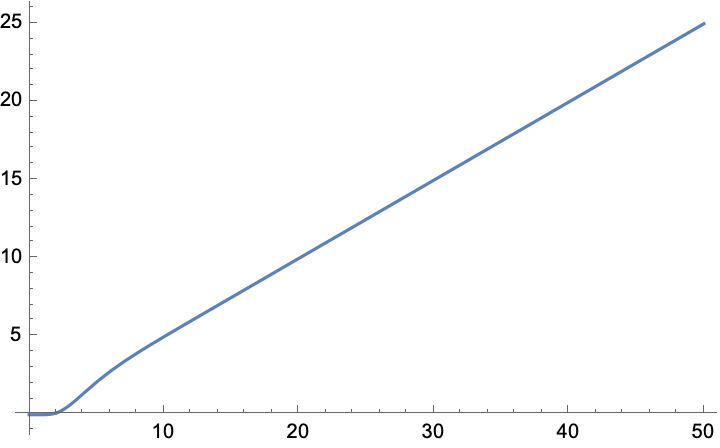
\includegraphics[scale=0.5]{q2a1.png}
				\end{center}
				Note that this plot looks approximately linear at high \(T\), but starts deviating 
				from it at lower \(T\). This makes sense, since this is the order where we can no longer 
				ignore the discretization of charge. As for \(Q^2\):
				\begin{center}
					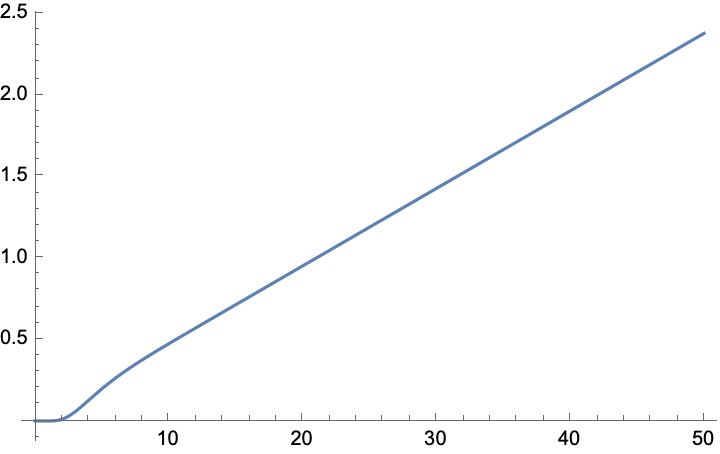
\includegraphics[scale=0.5]{q2a2.png}
				\end{center}
				The plot is the same shape, because we can calculate \(Q^2 = 2CE\). Again, notice the linear 
				relationship at high \(T\), and the fact that it breaks down at low \(T\) since we can't ignore 
				charge discretization.
			\end{solution}
		\item Derive the temperature scale $T \lesssim T_Q$, where charge quantization becomes important; \(T_Q\)
			should depend on \(C, e, k_B\).

			\begin{solution}
				From part (a), we calculated \(Z\) using the integral \(\int P(Q) dQ\), whereas in part (b) 
				we're told that the actual \(Z\) should be calculated as a discrete sum. Therefore, the 
				approximation as an integral breaks down when \(\Delta Q\) is comparable to the standard 
				deviation of the probability distribution -- as this is where we start to get large discrepancies
				in the calculated values. The standard deviation can be calculated as:
				\[
					\Delta Q = \mean{Q^2} - \mean Q = C k_B T 
				\] 
				And $T_Q$ occurs when \(\Delta Q \sim e\), so we have:
				\[
				\sqrt{C k_BT}  = e \implies T_Q = \frac{e^2}{k_B C}
				\] 
			\end{solution}
		\item When a large charge is placed on a capacitor, non-linear effects become important. We can 
			heuristically model their effect by assuming 
			\[
			E(Q) = \frac{Q^2}{2C} + gQ^4
			\] 
			Obtain an inequality of the form \(T_g \lesssim T\) above which you expect the non-linear term will 
			cause significant corrections to the equipartition theorem. \(T_g\) may depend on \(C, k_B, g\).

			\begin{solution}
				From the textbook, we know that the equipartition theorem fails when the average energy 
				is on the order of \(kT\). To calculate \(\mean{E}\), we first calculate the partition 
				function:
				\[
				Z(\beta) = \iinf e^{-\beta \left( \frac{Q^2}{2C} + gQ^4 \right) } dQ
				\] 
				Mathetmatica gives:
				\[
				Z(\beta) = \sqrt{\frac{2\pi C}{\beta}} e^{-\beta gQ^4}
				\] 
				So now we can calculate $\mean E$:
				\[
					\mean E = -\pdv{\beta} \ln Z = -\pdv{\beta} \ln \left( e^{-\beta gQ^4} \sqrt{\frac{2\pi C}{\beta}}  \right) 
				\] 
				Again, Matheamtica comes to the rescue here, and gives us:
				\[
				\mean E = \frac{1}{2\beta} + gQ^4 = \frac{k_BT}{2} + gQ^4
				\] 
				Therefore, when equipartition theorem fails, this is on the order of \(kT\) :
				\[
				\frac{1}{2\beta} + gQ^4 = k_BT \implies T = \frac{2gQ^4}{k_B}
				\] 
			\end{solution}
		\item For the same \(C\) discussed in part b, and \(g = \frac{k_B 0.1 \ \mathrm K}{e^4}\), numericaly 
			obtain plots for \(E(T) / k_B\) and \(Q^2(T) / e^2\) for \(0 < T < 100\) K, and compare with 
			equipartition. Can you explain the sign of the deviation?

			\begin{solution}
				To do this problem, I'd plot \(E(T)\) by computing:
				\[
				E(T) = \frac{1}{Z} \iinf e^{-\beta \left( \frac{Q^2}{2C} + gQ^4 \right) }\left( \frac{Q^2}{2C} + gQ^4 \right) dQ 
				\] 
				but unfortunately I ran out of time before I could plot anything. I'd do the same with 
				\(Q^2(T)\) :
				\[
				Q^2(T) = \frac{1}{Z} \iinf e^{-\beta\left( \frac{Q^2}{2C} + gQ^4 \right)} Q^2 dQ
				\] 
				again, I ran out of time :(.
			\end{solution}
	\end{enumerate}
	\pagebreak
	\section*{Problem 2}
	Consider the following simple model for a spring. It consists of a linear chain with \(N\) links for 
	\(N\) large, with temperature \(T\). Each link can either be aligned with the chain, in which case it 
	contributes a length \(a\) to it, or perpendicular to the chain, in which case it does not contribute 
	any length. Suppose the string is subject to a tension \(F\), so that turning a perpendicular link to 
	the aligned position costs energy \(Fa\). Compute
	\begin{enumerate}[label=\alph*)]
		\item The entropy of the chain as a function of its total length \(L\).

			\begin{solution}
				For a chain of length \(L\), this means that there are \(\frac{L}{a}\) molecules that are aligned
				with one another, so out of the \(N\) particles, there are \({N \choose L / a}\) ways 
				this can be done, meaning that our multiplicity is calculated as:
				\[
					\Omega(L) = {N \choose L / a}
				\] 
				Therefore, our entropy is: 
				\[
					S(L) = k_B \ln {N \choose L/a} = k_B \left[ \ln N! - \ln \left( \tfrac{L}{a} \right) !
					- \ln \left( N - \tfrac{L}{a} \right)!\right]= k_B \left[ N \ln N - 
				\left( \tfrac{L}{a} \right) \ln \left( \tfrac{L}{a}\right) - 
			\left( N- \tfrac{L}{a} \right) \ln \left( N - \tfrac{L}{a} \right) \right] 
				\]
			\end{solution}
		\item The length of the chain \(L\) as a function of \(T\), both in the microcanonical and the 
			canonical ensemble.

			\begin{solution}
				First we'll tackle the microcanonical ensemble. Given a length \(L\), this means that the 
				system has energy \(E = Fa \frac{L}{a} = FL\). Now, we have the following relation for 
				temperature:
				\[
					\frac{1}{T} = \pdv{S}{E} = \pdv{S}{L} \pdv{L}{E} = \pdv{S}{L} \left( \pdv{E}{L} \right)^{-1}
				\] 
				Firstly, we have \(\pdv{E}{L} = F\), so we just need to calculate \(\pdv{S}{L}\) :
				\begin{align*}
					\pdv{S}{L} &= k_B \pdv{L} \left[ N \ln N - \left( \frac{L}{a} \right) \ln \left( \frac{L}{a} \right) - \left( N - \frac{L}{a} \right) \ln \left( N - \frac{L}{a} \right)  \right]  \\
					&= k_B \left[ -\frac{1}{a}\ln \left( \frac{L}{a} \right) - \frac{L}{a}\frac{1}{L / a} \frac{1}{a} - \left( -\frac{1}{a} \right) \ln \left( N - \frac{L}{a} \right) - \left( N - \frac{L}{a} \right) 
					\frac{1}{N - L / a} \left( -\frac{1}{a} \right) \right]  \\
					&= \frac{k_B}{a}\left[ \ln \left( N - \frac{L}{a} \right) - \ln \left( \frac{L}{a} \right)  \right]  
				\end{align*}
				Therefore, we have:
				\[
				\frac{1}{T} = \frac{k_B}{a}\ln \left( \frac{Na}{L} - 1 \right) \frac{1}{F} \implies 
				L(T) = \frac{Na}{e^{Fa / k_BT} + 1}
				\] 
				Now for the canonical emsemble. To do this, we first have to find the partition function 
				\(Z\). To do this, we first consider the partition function for a single 
				link:
				\[
					Z_1 = e^{-\beta F(0)} + e^{-\beta F a} = 1 + e^{-\beta Fa}
				\] 
				To calculate the length using this formulation, we calculate \(\mean L\), which we can 
				write \(\mean L = N \mean{\ell}\), where \(\mean{\ell}\) denotes the average length 
				for a single unit. Therefore we have:
				\begin{align*}
					\mean L = N \mean \ell &= N \frac{e^{-\beta F(0)} \cdot 0 + ae^{- \beta F a}}{1 + e^{-\beta Fa}}\\
										   &= \frac{Nae^{- \beta Fa}}{1 + e^{- \beta Fa}} \\
										   &= \frac{Na}{1 + e^{\beta Fa}} 
				\end{align*}
				Note that this is the exact same expression as what we had in the microcanonical 
				ensemble, matching the fact that the theory is consistent. 
			\end{solution}
	\end{enumerate}
	Recall that the microcanonical ensemble we fix the energy of the system (or equivalently its length). On 
	the other hand, in the canonical ensemble we fix the temperature (i.e. we only demand that the energy 
	takes the macroscopic value on average). Do your results agree in the thermodynamic limit?
	\begin{enumerate}[label=\alph*), resume]
		\item Show that for high temperatures the spring satisfies Hooke's law. What is the spring 
			constant? 

			\begin{solution}
				For the question about the thermodynamic limit, note that we were only able to come to our 
				expression in the microcanonical ensemble when Stirling's approximation works, which is 
				in the regime of large \(N\). This is exactly the thermodynamic limit, so our results do agree. 

				Now, given \(L(T)\) (from the result of the previous problem), we can first solve for \(F\), 
				which gives us (after some algebra):
				\[
				F = \frac{1}{\beta a} \ln \left( \frac{Na}{L} - 1\right)
				\] 
				Now, we treat \(F\) as a function of \(L\), and do a Taylor expansion in \(L\). Notice that 
				in the high temperature limit of \(L(T)\), then we have \(L \to \frac{Na}{2}\), so this 
				suggests that when we expand \(F\) in \(L\), we substitute \(L = \frac{Na}{2}\) after the 
				Taylor expansion, which gives:
				\begin{align*}
					F(L + \Delta L) &= \frac{1}{\beta a}\left[ \ln \left( \frac{Na}{Na / 2} - 1 \right) 
					\frac{1}{ \frac{Na}{L} - 1} \left( -\frac{Na}{L^2} \right) \Delta L\right]  \\
					&= \frac{1}{\beta a}\left[ \frac{L}{Na - L} \left( -\frac{Na}{L^2} \right) \Delta L \right]  \\
					&= -\frac{4kT}{Na^2} \Delta L 
				\end{align*}	
				This suggests that our spring constant is \(\kappa = \dfrac{4kT}{Na^2}\). 
			\end{solution}
	\end{enumerate}
	\pagebreak
	\section*{Problem 3} 
	Recall the system we studied in the second problem in Homework 3. In this system we had \(N\) 
	distinguishable particles, each labelled by an integer \(i = 1, \dots, N\). Each of these particles could 
	have a spin with three possible values \(s_i = 0, \pm 1\). Furthermore, the energy of the system was 
	\[
		E = D \sum_{i = 1}^{N} s_i^2
	\] 
	for some constant \(D > 0\). In other words, each of the particles naturally wants to have spin \(s_i = 0\), 
	for the other two possibilities \(s_i = \pm 1\) cost energy \(D\). The purpose of this problem is to revisit
	this system in the canonical ensemble, and in particular we see that we can recover quantities that were 
	asked in HW3 in a much simpler way!
	\begin{enumerate}[label=\alph*)]
		\item Compute the canonical partition function of this system. Hint: Recall that the canonical partition
			function of non-interacting systems factorizes.

			\begin{solution}
				First, we can calculate the canonical partition function for a single spin: 
				\[
					Z_1 = e^{-\beta(0)} + 2e^{-\beta D}
				\] 
				Note that the second term is multiplied by 2 due to our degeneracy that \(s_i = \pm 1\) both 
				contribute energy \(D\). Then, since the particles are non-interacting, this means 
				we can just exponentiate:
				\[
				Z = Z_1^{N} = (1 + 2e^{-\beta D})^{N}
				\] 
			\end{solution}
		\item From the canonical partition function, obtain the energy of the system as a function of 
			temperature. 

			\begin{solution}
				To calculate \(\mean E\), we use the relation \(\mean E = -\pdv{\beta} \ln Z\), so carrying 
				out the algebra:
				\begin{align*}
					\mean E &= -\pdv{\beta} N \ln \left( 1 + 2e^{-\beta D} \right) \\
					&= -\frac{N}{1 + 2e^{-\beta D}} (-2D)e^{-\beta D} \\
					&= \frac{2ND e^{-\beta D}}{1 + 2e^{-\beta D}} 
				\end{align*}
			\end{solution}
		\item Using the canonical partition function, obtain the free energy and entropy of the system, both 
			as functions of temperature. Discuss the high and low temperature 
			behavior of entropy. 

			\begin{solution}
				We begin by calculating the free energy, using the relation that \(F = -k_BT \ln Z\). 
				So this means that:
				\[
				F = -k_BT \ln \left( 1 + 2e^{-\beta D} \right)^{N} = -N k_BT \ln\left( 1 + 2e^{-\beta D} \right) 
				\] 
				Now, to calculate entropy, remember the thermodynamic identity for the free energy:
				\[
				dF = -S dT - P dV + \mu dN
				\] 
				This means that \(\pdv{F}{T} = -S\), so we have to take the derivative of this expression 
				with respect to \(T\). After some algebra, we get:
				\[
				S = Nk_B \ln \left( 1 + 2e^{-\beta D} \right) + 
				\frac{Nk_BT}{1 + 2e^{-\beta D}}2e^{-\beta D} \cdot \frac{-D}{k_BT^2}
				\] 
				which, after some simplification with the help of our good friend Mathematica, 
				we get:
				\[
				S = Nk_B \ln\left( 1 + 2e^{-\beta D} \right) + \frac{2ND k_B}{T(2 + e^{\beta D})}
				\] 
				With the entropy computed, now we can discuss the high and low temperature limits. 
				At high \(T\), the second term goes to 0, so we're left with 
				\[
				S = Nk_B \ln (1 + 2e^{-D / kT}) = Nk_B \ln 3
				\] 
				this matches what we got in homework 3. For the low temperature limit, the first term 
				goes to zero, so we're left with the second term:
				\[
				S = \frac{2ND k_B}{T\left( 2 + e^{\beta D} \right) }
				\] 
				As \(T \to 0\), we see that \(\frac{2ND k_B}{T}\) blows up, but at the same time 
				\(\frac{1}{2 + e^{ D / kT}}\) goes to zero. Since the latter term is exponential in 
				\(T\), this means that it goes to zero faster than the former, so the limit 
				as a whole goes to zero, which matches what we derived in homework 3. 
			\end{solution}
	\end{enumerate}	
.\end{document}

